% Urban Flighter technical report (preprint-style).
% Compile: tectonic urban_flighter.tex
\documentclass[11pt]{article}
\usepackage[margin=1in]{geometry}
\usepackage{times}
\usepackage{graphicx}
\usepackage{booktabs}
\usepackage{amsmath,amssymb}
\usepackage{hyperref}
\usepackage{xcolor}
\usepackage{caption}
\usepackage{authblk}

\hypersetup{
  colorlinks=true,
  linkcolor=black,
  citecolor=black,
  urlcolor=blue
}

\title{Urban Flighter: An Honest Urban-Air Simulator\\
with CFD-lite Hidden Flow and Policy-Visible Sensing}
\author{Jaewon Jang}
\affil{Inha University; VortexyAether}
\date{August 2026}

\begin{document}
\maketitle

\begin{abstract}
Urban Flighter is an open-source urban drone simulator that couples real OpenStreetMap (OSM) building geometry, forecast-model inlet wind, and a browser cockpit with a headless research environment.
The design goal is not a new Navier--Stokes solver.
It is an \emph{honest contract}: hidden urban-flow approximations may drive dynamics, energy, and metrics, while a policy or baseline may observe only mission context, known inlet wind, onboard relative-air estimates, and deterministic geometry LiDAR.
We document the three public flight views (2D, 3D Lite, True 3D Wind overlay), the potential-flow CFD-lite field with wall damping and empirical wake correction, and UrbanFlow Gym, a NumPy environment that is RL-ready but \textbf{not trained}.
A fully offline showcase case on a synthetic fixture shows the expected qualitative result: unconstrained goal-seeking collides, geometry-safe A* succeeds, and an inlet-aware heuristic is \emph{not} automatically energy-optimal.
\end{abstract}

\section{Introduction}

Urban air mobility and small-UAV routing need environments where buildings, wind, sensing, and energy interact.
Many simulators either hide those interactions behind game physics or leak privileged flow fields into the learning agent.
Urban Flighter takes a third position: keep the cockpit watchable, keep the geometry real when a city is loaded, and keep the research contract explicit.

The software is already a working full-stack prototype:
\begin{itemize}
  \item a FastAPI backend that fetches OSM footprints and Open-Meteo current conditions, then computes CFD-lite fields;
  \item a React/Three.js frontend with 2D and 3D flight, LiDAR-inspired returns, and a Gym episode inspector;
  \item a headless UrbanFlow Gym core with leakage guards and deterministic baselines.
\end{itemize}

This report is a \emph{system paper / technical report}, not a claim of a new turbulence model or a trained policy.
All quantitative numbers in Section~\ref{sec:showcase} are produced by
\texttt{scripts/run\_oss\_showcase.py} and stored under \texttt{docs/showcase/}.

\section{Related systems and positioning}

AirSim, FlightGoggles, and related aerial simulators emphasize photorealism or vehicle dynamics.
Standalone CFD packages emphasize field accuracy but are not interactive flight products.
Urban Flighter sits between them: OSM-scale urban geometry, cheap hidden flow, and an RL-shaped observation contract.

Closest internal relatives are the project's own AeroJAX 2D incompressible Navier--Stokes snapshots (optional offline engine) and the browser CFD-lite B grid used for flyable dynamics.
The public cockpit does \emph{not} treat bundled True 3D $u/v/w$ streamlines as the flyable field.

\section{System architecture}

\paragraph{Backend.}
\texttt{backend/} serves geometry, weather, and flow.
\texttt{/flow-fields/2d} is the primary live endpoint: a streamfunction / potential-flow-ish grid with wall damping and an empirical wake correction (``CFD-lite B'').
Successful non-empty responses are registered as an immutable content-addressed snapshot \texttt{urbanflow.live\_scenario.v1}.

\paragraph{Frontend.}
Three public modes:
\begin{itemize}
  \item \textbf{2D}: north-up canvas, 120\,Hz fixed-step motion, swept-circle clearance, 180-ray scan.
  \item \textbf{3D Lite}: metre-scale quadcopter, same horizontal live grid, building/ground LiDAR, presentation-only city dressing.
  \item \textbf{True 3D Wind}: the same flyable city plus a bundled 3D potential-flow $u/v/w$ overlay (Gangnam demo). Overlay $\neq$ flight dynamics.
\end{itemize}

\paragraph{Energy proxy.}
Unless a more detailed motor model is requested, step energy uses relative airspeed
\begin{equation}
  e_t = \lVert \mathbf{v}_{\mathrm{ground},t} - \mathbf{w}_{\mathrm{local}}(\mathbf{x}_t,t) \rVert^2 \Delta t.
\end{equation}
The local wind $\mathbf{w}_{\mathrm{local}}$ is a hidden sample. The actor may receive only an onboard estimate and the known inlet.

\paragraph{Honesty labels.}
The product UI and this paper use the same vocabulary:
CFD-lite $\neq$ Navier--Stokes;
SIM odometry / no loop closure;
UrbanFlow Gym / NOT TRAINED;
full flow access = NO.

\section{CFD-lite hidden dynamics}

\subsection{Potential-flow slice}
A 2D slice solves a discrete Laplace problem for a streamfunction or potential on a masked grid, then recovers $\mathbf{u}=\nabla\phi$ (or the streamfunction equivalent).
Inlet / far-field velocity is prescribed; building cells are solid.
This produces cheap acceleration around corners (Fig.~\ref{fig:flow}).

It cannot represent viscous separation, vortex shedding, or turbulence.
Empirical wall damping and downstream wake patches are therefore added for drone-risk realism and must be labelled as such.

\subsection{True 3D overlay}
A voxel potential-flow field supplies $u,v,w$ streamlines for visualization.
The flyable 3D aircraft still samples the live horizontal CFD-lite grid.
No Navier--Stokes residual is claimed for either field.

\begin{figure}[t]
  \centering
  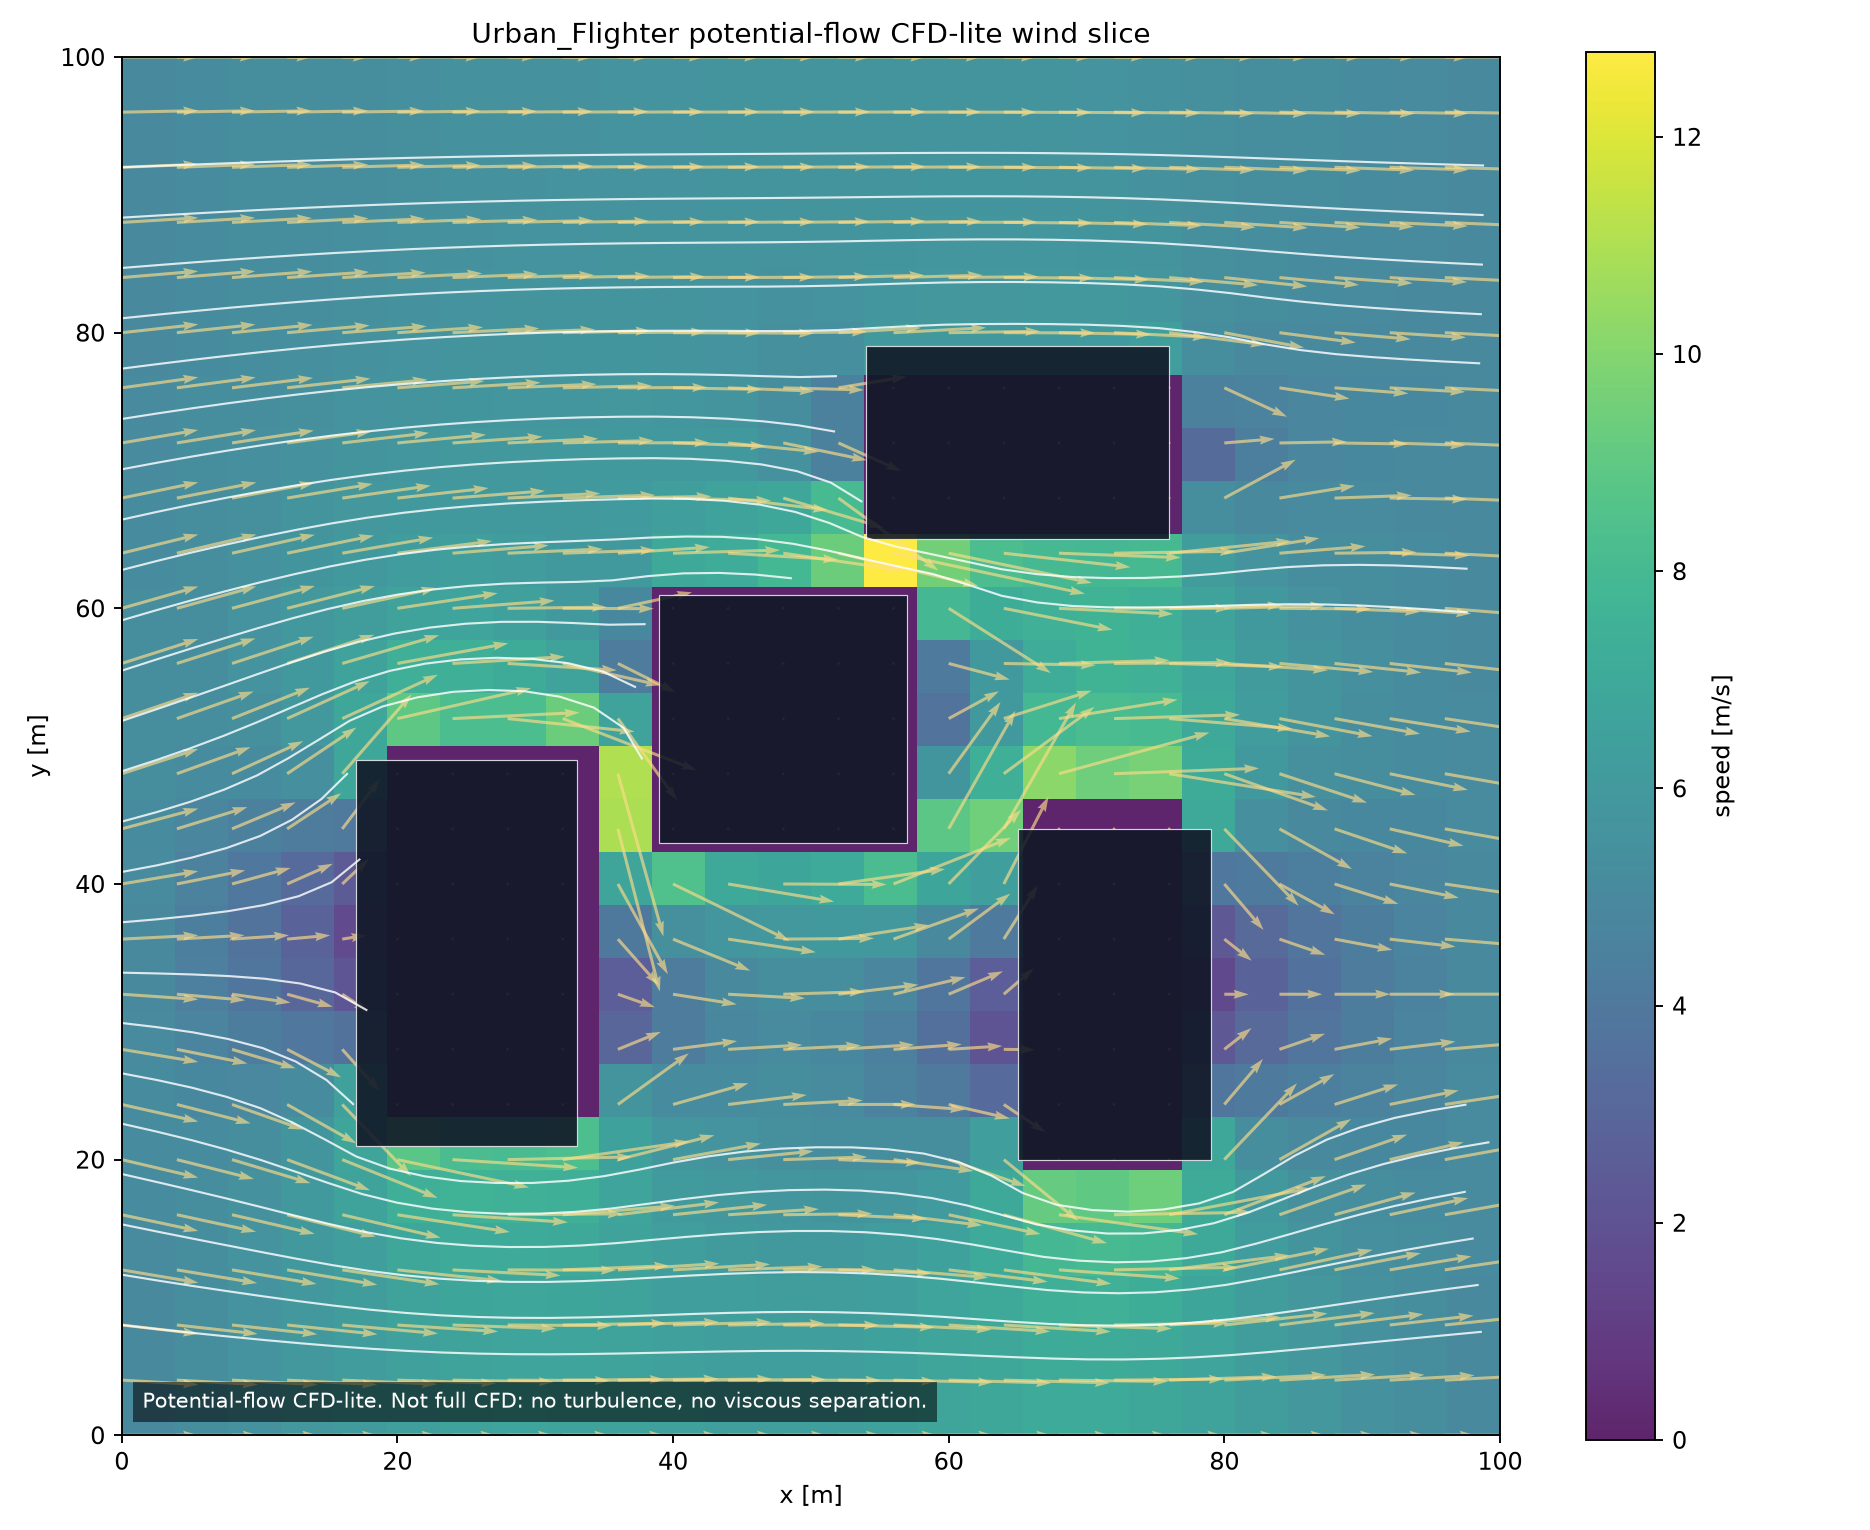
\includegraphics[width=0.92\linewidth]{figures/fig_potential_flow.png}
  \caption{Offline toy-city potential-flow CFD-lite showcase.
  Five prisms, 5\,m/s westerly inlet, $26\times 26$ grid, 348 iterations, residual $9.84\times 10^{-5}$.
  Mean speed $4.96$\,m/s, max speed $12.8$\,m/s.
  Not Navier--Stokes.}
  \label{fig:flow}
\end{figure}

\section{Sensing and the actor contract}

Frontend LiDAR prototypes use a frozen five-value-per-ray layout
\[
  (d_x,d_y,d_z,\hat{r},h),
\]
local direction, normalized range, and hit flag.
3D default: 600 Fibonacci-sphere samples, 120\,m max range.
2D default: 180 rays, 180\,m.

UrbanFlow Gym uses a separate 33-scalar actor observation: own motion, goal context, fixed-angle geometry LiDAR, known inlet, previous action, and an onboard relative-air estimate.
Automated leakage guards reject full grids, exact wakes, future samples, and provider objects in the actor channel.
A privileged critic helper exists and is never returned by \texttt{reset}/\texttt{step}.

\section{UrbanFlow Gym}
\label{sec:gym}

The core environment is NumPy-only.
Gymnasium / Stable-Baselines3 / Torch are optional extras and are not imported on the default path.
Action is a bounded 2D local-guidance command in the vehicle frame, not motor RPM.

Three deterministic baselines share the public mission context only:
\begin{enumerate}
  \item \textbf{Direct goal}: steer toward the goal (no obstacle planner).
  \item \textbf{Shortest path}: geometry-safe A* + waypoint tracking.
  \item \textbf{Inlet-aware}: A* with known-inlet feed-forward. Still \emph{not} privileged-grid access.
\end{enumerate}

Live evaluation binds to the exact UI-registered OSM scenario.
The showcase below uses the synthetic rectangular fixture so that open-source CI needs no network.

\section{Showcase case}
\label{sec:showcase}

Command (repo root, no network):
\begin{verbatim}
PYTHONPATH=backend python scripts/run_oss_showcase.py
\end{verbatim}
Artifacts: \texttt{docs/showcase/}.

\subsection{Potential-flow field}
Toy city, five buildings, inlet from $270^\circ$ at 5\,m/s (Fig.~\ref{fig:flow}).

\subsection{Baseline comparison}
Three held-out fixture seeds $\{10007,10009,10037\}$, horizon 240 steps, $\Delta t=0.25$\,s.
Table~\ref{tab:eval} and Figs.~\ref{fig:traj}--\ref{fig:metrics}.

\begin{table}[t]
\centering
\caption{UrbanFlow Gym synthetic-fixture evaluation.
Policy status: NOT TRAINED.
Privileged flow access: false.
Hidden dynamics: synthetic potential-flow-ish wake proxy, not Navier--Stokes.}
\label{tab:eval}
\begin{tabular}{lcccc}
\toprule
Baseline & Success & Mean path (m) & Rel-air energy & Collision eps. \\
\midrule
Direct goal & $0/3$ & $23.5$ & $180$ & $3/3$ \\
Shortest-path A* & $3/3$ & $142.1$ & $1236$ & $0/3$ \\
Inlet-aware A* & $3/3$ & $141.9$ & $1303$ & $0/3$ \\
\bottomrule
\end{tabular}
\end{table}

\begin{figure}[t]
  \centering
  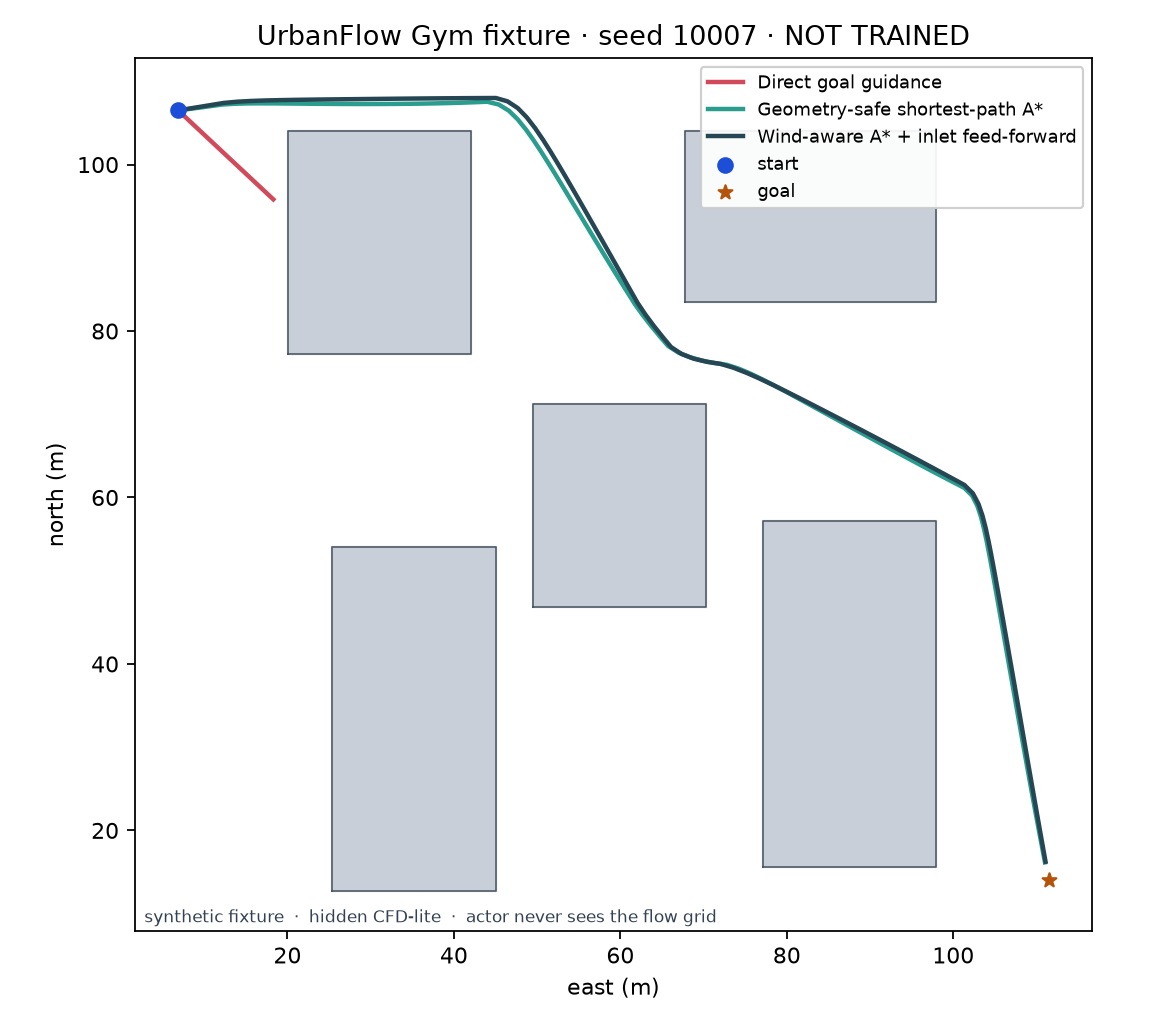
\includegraphics[width=0.88\linewidth]{figures/fig_trajectories.png}
  \caption{Seed 10007 rollouts on the synthetic fixture.
  Direct goal collides.
  Both planners reach the goal without building hits.
  Actor observation dimension is 33.}
  \label{fig:traj}
\end{figure}

\begin{figure}[t]
  \centering
  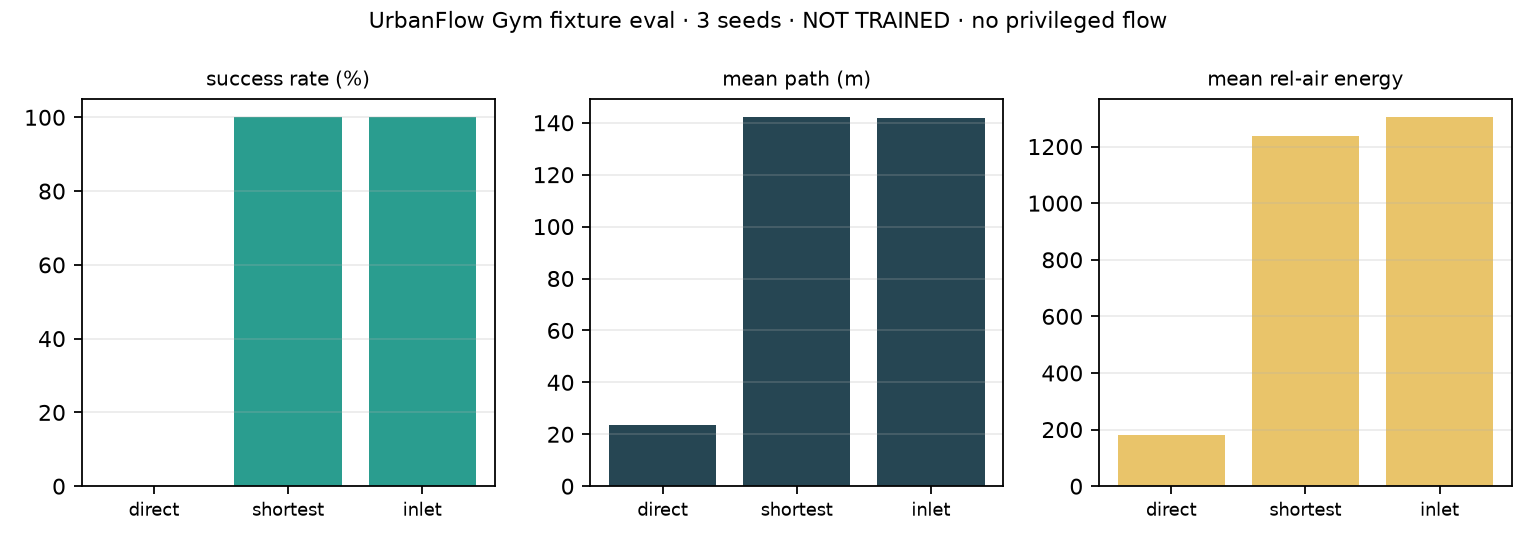
\includegraphics[width=\linewidth]{figures/fig_metrics.png}
  \caption{Aggregate fixture metrics.
  Inlet-aware is not energy-better than shortest path on this set; we report the regression rather than force a narrative.}
  \label{fig:metrics}
\end{figure}

\paragraph{Reading.}
The showcase is a \emph{contract test}, not a claim that wind-aware planning wins.
A successful OSS demo must show (i) collisions when geometry is ignored, (ii) success when it is not, (iii) no privileged-grid leakage, and (iv) honest labels.

\section{Limitations}

\begin{itemize}
  \item CFD-lite and voxel potential flow are not LES/RANS/DNS.
  \item True 3D Wind is a visualization overlay.
  \item LiDAR and rolling maps are simulator rays plus odometry, not hardware SLAM.
  \item No PPO/SAC training is shipped; ``RL-ready'' $\neq$ ``trained.''
  \item Live OSM/weather paths need network; the committed showcase does not.
  \item Presentation trees/roads never enter physics, sensors, Gym, or scenario hashes.
\end{itemize}

\section{Reproducibility}

\begin{itemize}
  \item Code: \url{https://github.com/VortexyAether/Urban_Flighter}
  \item License: MIT.
  \item Showcase seed and command: Section~\ref{sec:showcase}.
  \item Evaluation id of the reported JSON: \texttt{24ec026f3352e4f9}.
\end{itemize}

\section{Conclusion}

Urban Flighter is released as an open urban-air research cockpit: real cities when requested, cheap hidden flow, and a deliberately narrow actor contract.
The first public case study is intentionally boring and checkable.
That is the point.

\appendix
\section{Software map}
\texttt{backend/} FastAPI and CFD-lite services;
\texttt{backend/urbanflow\_gym/} headless env;
\texttt{frontend/} React 19 + Three.js;
\texttt{scripts/run\_oss\_showcase.py} this paper's case;
\texttt{CLAUDE.md} contributor contract.

\end{document}
